\documentclass[10pt]{article}
\usepackage{float}
\RequirePackage{eso-pic}
\usepackage{caption}
\captionsetup[table]{labelformat=empty}



\usepackage{geometry}
\geometry{
a4paper,
left=11mm,
right=14mm,
top=37mm,
bottom=14mm,
}



\usepackage{colortbl}
\usepackage{fontspec}
\setmainfont[Ligatures=TeX]{Calibri}



\newcommand\BackgroundPic{%
\put(0,0){%
\parbox[b][\paperheight]{\paperwidth}{%
\vfill
\centering
\includegraphics{MBIE_generic_background.pdf}%
\vfill
}}}



\begin{document}
\thispagestyle{empty}
\AddToShipoutPicture{\BackgroundPic}
\section*{Key Export Statistics\footnotemark - Chicken\footnotemark }
\today\\
\begin{table}[ht]
\centering
{\scriptsize
\begin{tabular}[t]{p{1.8cm}>{\hfill}p{1.4cm}>{\hfill}p{1.4cm}>{\hfill}p{1.6cm}>{\hfill}p{1.9cm}>{\hfill}p{2cm}>{\hfill}p{1.9cm}>{\hfill}p{1.5cm}}
 \textbf{Country} & \textbf{Yearly Qty} & \textbf{Yearly Value} & \textbf{Yearly Price} & \textbf{3Year CAGR(Qty)} & \textbf{3Year CAGR(Value)} & \textbf{3Year CAGR(Price)} & \textbf{Price Elasticity} \\
\hline
Australia & 6,874 & 41.7 & \$6.1 & 16.6\% & 2.2\% & -12.3\% & -1.3 \\  
P.N.G & 2,559 & 7.9 & \$3.1 & 87.9\% & 93.2\% & 2.8\% & 30.9 \\  
Vanuatu & 1,146 & 2.7 & \$2.4 & 117.9\% & 103.7\% & -6.5\% & -18.1 \\  
Fiji & 1,240 & 2.3 & \$1.8 & -2.6\% & -8.2\% & -5.8\% & 0.5 \\  
Solomon Islands & 555 & 1.3 & \$2.4 & 91.2\% & 93.5\% & 1.2\% & 77.5 \\  
U.A.E & 262 & 0.6 & \$2.5 & -22\% & -27.4\% & -6.9\% & 3.2 \\  
Other & 478 & 1.5 & \$3.2 & -58.8\% & -67.7\% & -21.6\% & 2.7 \\  
Total & 13,114 & 58.1 & \$4.4 & 44.6\% & 14.2\% & -21\% & -2.1 \\  
\hline
\end{tabular}
}
\caption{\scriptsize Top 6 Chicken Markets for year ending November - 2015: Quantity('000 kg) Value(NZ\$Mill), Price and their last 3-Year Growth Rates}
\end{table}


\vspace{-0.7cm}



   \begin{figure}[H]
   \centering
    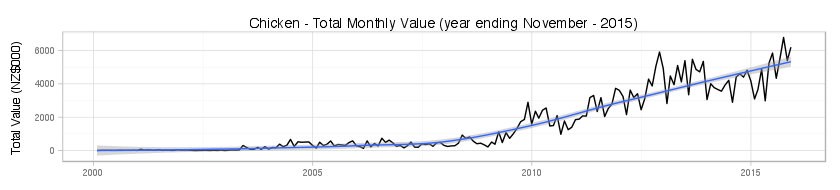
\includegraphics[scale=0.5]{../graphs/monthly_value/chicken_monthly_value.png} \
    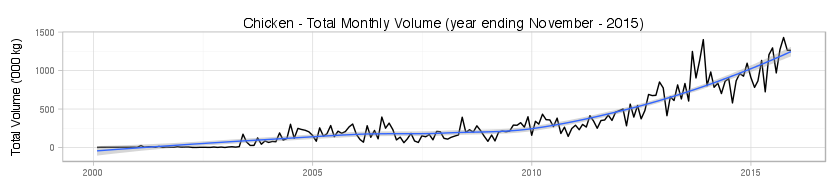
\includegraphics[scale=0.5]{../graphs/monthly_volume/chicken_monthly_volume.png} \
    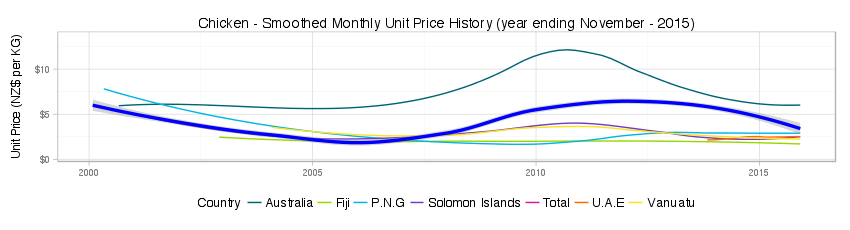
\includegraphics[scale=0.5]{../graphs/smoothed_price/chicken_smoothed_price.png} \
    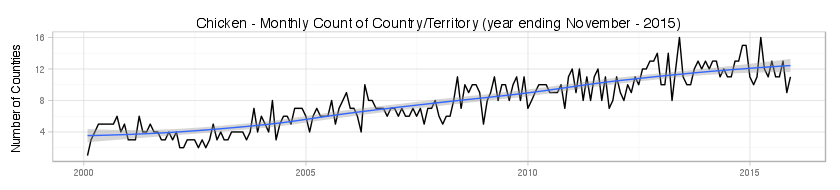
\includegraphics[scale=0.5]{../graphs/monthly_number_countries/chicken_monthly_count.png} \
    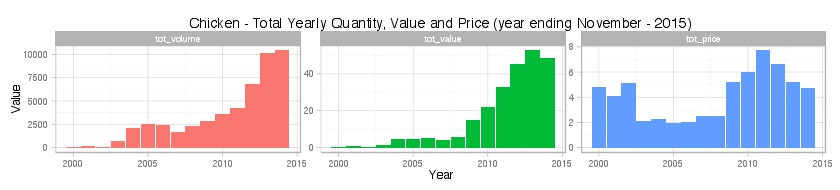
\includegraphics[scale=0.5]{../graphs/yearly_summary/chicken_yearly_summary.png} \
   \end{figure}



\footnotetext[1]{Source: Statistics New Zealand - Overseas Merchandise Trade}
\footnotetext[2]{Harmonised System Codes for Chicken starting with: 020714.}
\end{document}
